%*****************************************************************************************
%*********************************** First Chapter ***************************************
%*****************************************************************************************

\chapter{Introduction}  %Title of the First Chapter

\ifpdf
    \graphicspath{{Chapter1/Figs/Raster/}{Chapter1/Figs/PDF/}{Chapter1/Figs/}}
\else
    \graphicspath{{Chapter1/Figs/Vector/}{Chapter1/Figs/}}
\fi


A systems level understanding of biology has always been in the back
of the minds of biologists since it is this distributed information
processing that ultimately gives rise to phenotype and macroscopic
behaviour to sustain life. Perhaps the apparent great complexity at
which these systems operate or the lack of relevant experimental data
has made Biology as a discipline to focus its efforts on the
understanding of the information processing capabilities and inner
workings of the individual constituent components of these
systems. Relatively recent technological advances however have led to
an accumulation of a wealth of data sheding light into the interactions
between components, their dependencies and the constraints these
impose. While understanding the individual components, genes,
proteins, is still important these new data sources have led to a shift
of focus to the study of biological systems in their entirety. In
doing so we realised that the most important aspect of these systems
is not the inner workings of the individual components but rather the
interactions between them.

Traditionally biology has not used any formal methods to explain
things and perhaps that was not needed when we were dealing with
single entities. As the systems grew in size it became apparent that
some change in direction was needed to handle the increased complexity
and get a coherent story. Systems Biology tries to fill this gap by
bringing in practises from other more traditionally formal fields like
Mathematics, Physics, Computer Science(\citet{kitano2002systems, ideker2001new}).

Early attempts to capture the more complex picture painted by the
increase in the number of components were to use static diagrams to
capture the interactions and dependencies between them. These diagrams
have been widely used in Biochemistry and particularly in metabolism
since the species conversion process that takes place in metabolic
pathways can easily be seen as a path or paths through these diagrams going from
one metabolite to the next(see for example
Figure~\ref{fig:fa_synthesis_pathway}). Now these diagrams are very important and
they contain important knowledge about our understanding of the
operations of biological systems. There exist databases that contain our current
understanding of a particular system annotated with information from
different sources and these are particularly popular for metabolic
pathways (see \citet{kanehisa2000kegg},
\citet{pharkya2003review}). These static diagrams are an example of
bottoms-up approach in System Biology which is a data-driven process,
starting from some large experimental datasets we extract biological
information. This is in contrast to the top-down approach where
starting from detailed knowledge about a system we try to build a
mechanistic explanation of it(\citet{schneider2013understanding}). 

\begin{figure}[htbp!] 
\centering    
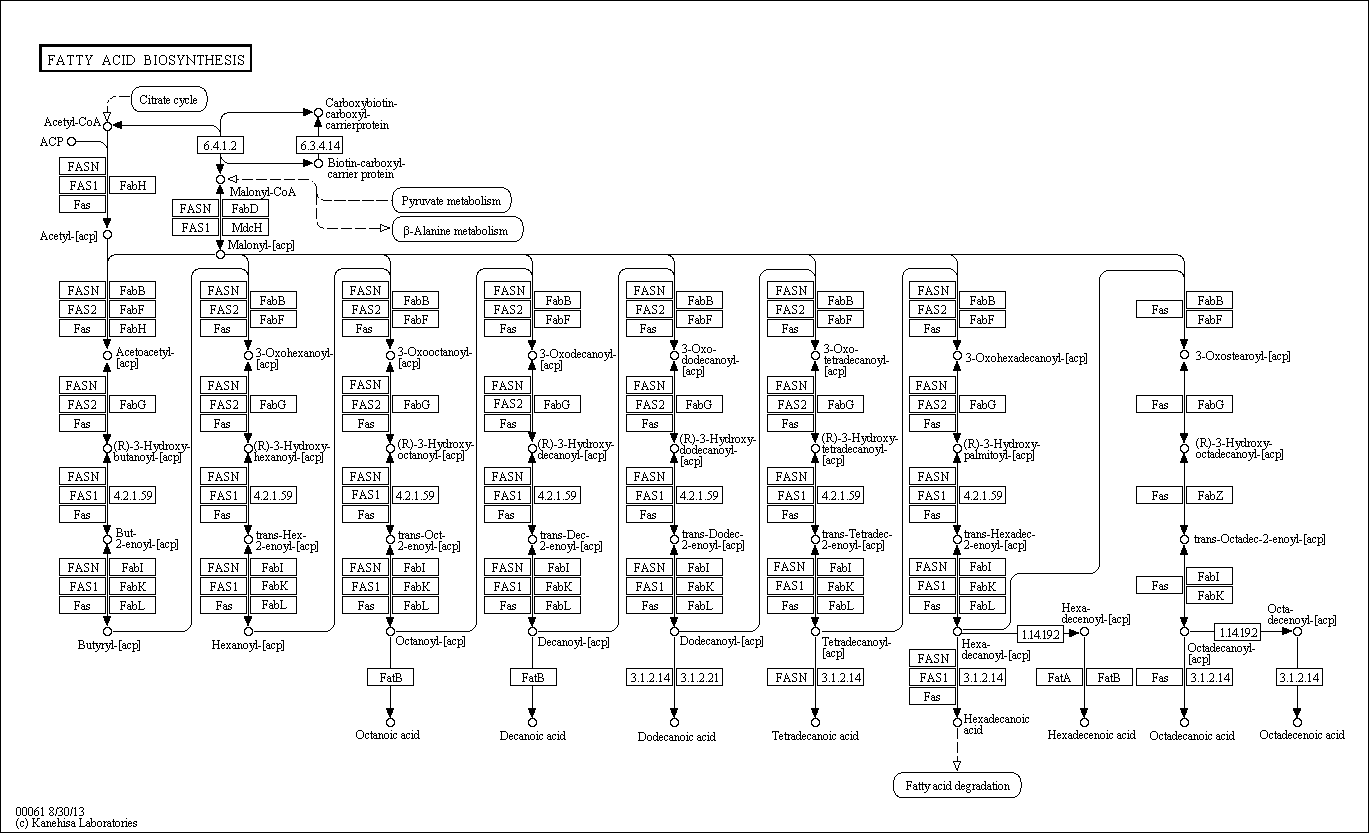
\includegraphics[width=1.0\textwidth]{fa_synthesis_pathway}
\caption[Fatty Acid synthesis pathway]{Fatty acid synthesis pathway
  captured by the standard diagrammatic language used to capture
  interactions between components in a biological system. This was
  taken from KEGG a database which contains current knowledge about
  the working of these systems(from experiments for example)
  integrated with data from multiple sources.}
\label{fig:fa_synthesis_pathway}
\end{figure}

Despite the importance of the bottom-up static diagrams they paint a
very static picture of the system which is not enough to gain a full
understanding of the system. What is often needed is a dynamic picture
of the system with a top-down mechanistic model to observe things that
are not possible from a static
picture like control mechanisms, dynamic interactions between
components over time, and dynamic responses to external stimuli.


\section{Dynamical systems theory and Flux Balance Analysis}
This need to look into dynamic behaviour led to Dynamical System
theory which based on its success in Physics has found its way in many
other fields. Dynamical system theory captures the relationship
between continuous quantities in difference-differential equations
which describe the evolution of state variables in terms of changes
in other state variables and even themselves thus capturing the
interaction element. Since the time of Newton and classical mechanics
,where these ideas originated, the toolbox of dynamical systems theory
has grown to include techniques for qualitative understanding of
system without the need to solve them either numerically or analytically.


\section{Challenge of lipid metabolism}



\section{Computational models in Biology}


\section{Outline of work}